\documentclass{esann}
%\usepackage[dvips]{graphicx}
\usepackage[pdftex]{graphicx}
\usepackage[latin1]{inputenc}
\usepackage{amssymb,amsmath,array}
\usepackage{scrextend}
\usepackage{hyperref}
\usepackage{multirow}
\usepackage{mathtools}
\usepackage{wrapfig}
\usepackage{natbib}
\usepackage{enumitem} 
%***********************************************************************
% !!!! IMPORTANT NOTICE ON TEXT MARGINS !!!!!
%***********************************************************************
%
% Please avoid using DVI2PDF or PS2PDF converters: some undesired
% shifting/scaling may occur when using these programs
% It is strongly recommended to use the DVIPS converters, and to submit
% PS file. You may submit a PDF file if and only if you use ADOBE ACROBAT
% to convert your PS file to PDF.
%
% Check that you have set the paper size to A4 (and NOT to letter) in your
% dvi2ps converter, in Adobe Acrobat if you use it, and in any printer driver
% that you could use.  You also have to disable the 'scale to fit paper' option
% of your printer driver.
%
% In any case, please check carefully that the final size of the top and
% bottom margins is 5.2 cm and of the left and right margins is 4.4 cm.
% It is your responsibility to verify this important requirement.  If these margin requirements and not fulfilled at the end of your file generation process, please use the following commands to correct them.  Otherwise, please do not modify these commands.
%
\voffset 0 cm \hoffset 0 cm \addtolength{\textwidth}{0cm}
\addtolength{\textheight}{0cm}\addtolength{\leftmargin}{0cm}

%***********************************************************************
% !!!! USE OF THE esannV2 LaTeX STYLE FILE !!!!!
%***********************************************************************
%
% Some commands are inserted in the following .tex example file.  Therefore to
% set up your ESANN submission, please use this file and modify it to insert
% your text, rather than staring from a blank .tex file.  In this way, you will
% have the commands inserted in the right place.

\begin{document}
%style file for ESANN manuscripts
\title{Choosing the Best Algorithm for an Incremental On-line Learning Task}

%***********************************************************************
% AUTHORS INFORMATION AREA
%***********************************************************************
\author{Viktor Losing$^1$$^2$ Barbara Hammer$^2$ and Heiko Wersing$^1$
%
%
% DO NOT MODIFY THE FOLLOWING '\vspace' ARGUMENT
\vspace{.3cm}\\
%
% Addresses and institutions (remove "1- " in case of a single institution)
1- HONDA Research Institute Europe GmbH,\\
Carl-Legien-Str. 30, 63065 Offenbach - Germany
%
% Remove the next three lines in case of a single institution
\vspace{.1cm}\\
2- Bielefeld University, Universitaetsstr. 25, 33615 Bielefeld - Germany
}
%***********************************************************************
% END OF AUTHORS INFORMATION AREA
%***********************************************************************

\maketitle

\begin{abstract}
Recently, incremental and on-line learning gained more attention 
especially in the context of big data and learning from data streams,
conflicting with the traditional assumption of complete data availability. Even though 
a variety of different methods are available, it often remains unclear which of them is suitable
for a specific task and how they perform in comparison to each other. 
We analyze the key properties of seven incremental methods representing different algorithm classes.
Our extensive evaluation on data sets with different characteristics gives an overview of the performance with respect to accuracy as well as model complexity,
facilitating the choice of the best method for a given application.
\end{abstract}

\section{Introduction}
Attention in the field of incremental learning has grown drastically in recent years which is caused by two major developments. The main reason is the rapidly increasing amount of data accumulation in fields such as health monitoring,
social networks, financial transactions or personalized web services \cite{ageOfBigData}, \cite{bigDataSurvey}, demanding for continuous large-scale, real-time processing. 
Another trend is to incorporate individual adaptation to customer habits and environments within smart home products \cite{Yang:2013:LLT:2493432.2493489}, \cite{Carolis:2015:ILD:2688469.2675063} requiring
skills such as efficient learning from few data.\\
A lot of ambiguity is involved regarding the definition of incremental and on-line learning in the literature. Some authors use them interchangeably, while others distinguish them in different ways. 
Additional terms such as lifelong- or evolutionary learning are also used synonymously. We define an incremental learning algorithm as one that generates on a given stream of training data $x_1,x_2,...,x_t$ a sequence of models $M_1,M_2,...,M_t$ and thereby meets
the following criteria:
\begin{itemize}[leftmargin=2em, topsep=0.3em, partopsep=0em, parsep=0em, itemsep=0em] 
\item $M_{t+1}$ adapts gradually based on $M_{t}$ without a complete retraining.
\item It preserves previously acquired knowledge and does not suffer from the effect of catastrophic forgetting. %\cite{french1999catastrophic}.
\item It has a limited stream memory.
\end{itemize}
We specify on-line learning algorithms as incremental learning algorithms which are additionally bounded in model complexity and run-time, capable of endless/lifelong learning on a device with restricted resources.\\
A variety of interesting incremental learning algorithms have been published but there is a lack of in-depth comparative studies. 
In this paper we contribute to fill this gap by analyzing the core attributes of seven popular methods. 
Experiments on diverse datasets assess their performance and provide guidance on their applicability for specific tasks. We focus solely on the classification of stationary datasets (i.e.\ we assume
the stream $x_1,x_2,...$ is i.i.d.) and not yet analyze the methods in context of concept drift. A recent overview of methods especially designed to deal with non-stationary environments is given in \cite{ditzler2015learning}. 

\section{Algorithms}
In the following we briefly describe all tested methods including Bayesian -, linear -, instance based models as well as ensembles and
neural networks.\\
\textbf{Incremental Support Vector Machine (ISVM)}, introduced in \cite{cauwenbergs01incrementaldecremental}, is the only exact incremental version of the SVM.  
%It is a lossless algorithm - generates the same model as the corresponding batch algorithm - given access to all previously seen data. 
A limited number of examples, so called ``candidate vectors'', which could be promoted to support vectors in the future, is additionally maintained.\\
%A smaller set of candidate vectors increases the probability of missing potential support vectors.\\
\textbf{On-line Random Forest (ORF)}\cite{5457447} is an incremental version of the Extreme Random Forest. 
A predefined number of trees grow continuously by adding splits whenever enough samples are gathered within one leaf.
Tree ensembles are very popular, due to their high accuracy, simplicity and parallelization capability. \\
\textbf{Incremental Learning Vector Quantization (ILVQ)} extends the Generalized Learning Vector Quantization (GLVQ) to a dynamically growing model by continuous insertion of new prototypes. 
We introduced a superior prototype placement strategy in \cite{7280610} minimizing the loss on a window of recent samples. Metric learning, as described in \cite{Schneider:2009:ARM:1737743.1737754}, %\cite{bunte2012limited} 
can also be applied.\\
\textbf{Learn++ (LPP)}\cite{983933} processes incoming samples in chunks with a predefined size. For each chunk an ensemble of base classifiers is trained and combined through weighted majority voting to an ``ensemble of ensembles``.
%Similar to AdaBoost, each classifier is trained with a subset of chunk examples drawn according to a distribution, ensuring a higher sample probability for misclassified inputs.
Chunk-wise trained models have by design an adaption delay depending on the chunk size.\\
\textbf{Incremental Extreme Learning Machine (IELM)} reformulates the batch ELM least-squares solution into a sequential scheme \cite{4012031}. As the batch version it drastically reduces the training complexity by 
randomizing the input weights. The network is static and the number of hidden neurons has to be predefined.\\
\textbf{Gaussian Naive Bayes (GNB)}
fits one axis-parallel Gaussian distribution per class and uses them as likelihood estimation in the Naive Bayes algorithm \cite{Chan:1979:UFP:892239}. 
The algorithm is lossless, i.e.\ it generates the same model as the corresponding batch algorithm, and independent from the training order.\\
\textbf{Stochastic Gradient Descent (SGD)} is an efficient method for learning a linear, discriminative model by minimizing a convex loss function. Revived recently in the context of
large-scale learning \cite{bottou2010large} it performs especially well for sparse, high-dimensional data as often encountered in the domain of text classification. 
%XXVLWe used solely the hinge loss function for our experiments.
%\footnote{We extended the code \url{https://github.com/diehl/Incremental-SVM-Learning-in-MATLAB} for multi-class classification by the one vs. all scheme.}
%\footnote{Code at \url{https://github.com/amirsaffari/online-multiclass-lpboost}}
%\footnote{\label{ditzler} Code at \url{https://github.com/gditzler/IncrementalLearning}, which uses CART \cite{cart84} as weak classifier.}
%\footnote{Code at \url{http://www3.ntu.edu.sg/home/egbhuang/elm_codes.html}.}
%\footnote{\label{sklearn}Scikit-learn implementation \url{http://scikit-learn.org/}.}
\section{Experiments}


We used the implementations of the Scikit-learn package \cite{scikit-learn} for SGD and GNB. All the others are derived from the code of the respective authors.
Only publicly available datasets (see \cite{Lichman:2013}, \cite{CC01a}), predefining a fixed train-test-split, were used to enable reproducibility and comparability of our results. 
Table \ref{tab:datasets} gives the main attributes of the selected datasets. Artificial and real world problems are included, differing widely in the number of classes, instances and dimensions.
Links to all implementations and datasets are available at \url{https://github.com/vlosing/Online-learning}.
\def \tCol{-8pt}

\subsection{Hyperparameter setting}
\begin{wraptable}{r}{5.5cm}
\def\arraystretch{0.9}
\footnotesize
\centering
\begin{tabular}{@{}r<{\hspace{-3pt}}|@{ }c<{\hspace{\tCol}}c<{\hspace{\tCol}}c<{\hspace{\tCol}}c<{\hspace{\tCol}}c<{\hspace{\tCol}}@{}}
\textit{Dataset} & \#Train&\#Test&\#Feat.&\#Class\\\hline
\rule{0pt}{8pt}
Border & 4000 & 1000 & 2 & 3\\
Overlap & 3960 & 990 & 2 & 4\\
Letter & 16000 & 4000 & 16 & 26\\
Outdoor & 2600 & 1400 & 21 & 40\\
COIL & 1800 & 5400 & 21 & 100\\
DNA & 1400 & 1186 & 180 & 3\\
USPS & 7291 & 2007 & 256 & 10\\
Isolet & 6238 & 1559 & 617 & 26\\
MNist & 60000 & 10000 & 784 & 10\\
Gisette & 6000 & 1000 & 5000 & 2\\
\end{tabular}
\caption{The evaluated datasets.}
\label{tab:datasets}
\end{wraptable}
The model selection is varying in complexity depending on the parameter amount and type. 
Tree based models usually perform well out of the box, whereas the ISVM or ILVQ require an accurate, dataset dependent configuration of multiple parameters to deliver good results. The ISVM is
solely paired with the RBF kernel. We use the metric learning of ILVQ only for datasets with up to 250 dimensions.  The GNB algorithm is parameterless, hence no tuning is required at all. We minimize the hinge loss function with SGD and adjust only the learning rate. LPP requires the number of base classfier per chunk as well as 
the parameters of the base classifier itself (non-parametric Classification and Regression Trees). All parameter are set by Hyperopt \cite{bergstra2015} performing repeatedly a 3-fold cross validation on the training data.

\subsection{Measure of model complexity}
The algorithm implementations vary in the written programming languages as well as their efficiency. Therefore, we do not compare training- and run-time but instead we measure the model complexity
by counting the number of parameter required for the representation. This enables a comparison with respect to memory consumption. 
However, the models are fundamentally different so that this measure, even though there is some correlation, should not generally be equated with training- or run-time.
For instance, the $\mathcal{O}(\log l)$ run-time of tree based models, l being the number of leaves, make them incredible fast in comparison to instance based ones ($\mathcal{O}(d*i)$, for i
instances (e.g. prototypes, support vectors) with d dimensions).
Another example are the Extreme Random Trees deployed by the ORF algorithm. By introducing random splits they drastically reduce the training-time, but also require larger trees\cite{ert}.
We rather use this measure as an indicator to decide whether an algorithm struggles (unreasonable high amount of parameters) or is especially suited (sparse representation paired with high accuracy) for a given task. 
% \begin{eqnarray*}
% P_{Tree}(t)&=&splits(t)*3 + leaves(t)*2\nonumber\\
% P_{ORF}&=&\sum_{i=1}^{n} P_{Tree}(t_i)\nonumber\\
% P_{LPP}&=&\sum_{i=1}^{n} P_{Tree}(t_i) + n\nonumber\\
% P_{ISVM}&=&sv*(dim+1)+1\nonumber\\
% P_{ILVQ}&=&proto*(dim+1)+dim^2\nonumber\\
% P_{IELM}&=&dim*hneurons+hneurons*classes\nonumber\\
% P_{SGD}&=&\begin{dcases*}
%         dim+1  &$classes=2$\\
%         dim * classes + classes &$classes>2$
%         \end{dcases*}\\
% P_{GNB}&=&classes*dim*2.\nonumber\\
% \end{eqnarray*}
% Most are self-explanatory, but we explain the measure for trees in detail.
% Each node needs one parameter to represent its parent, since the tree structure determines the sequence of splits. Each split 
% needs additionally one parameter for the dimension and one for its value. Leaves have to store also their label.\\ The complexities
% of all experiments are given in table \ref{tab:complexities}.

\subsection{Results}
%The different algorithms make a fair comparison quite challenging. 
The evaluation of GNB, ORF and SGD is straightforward since these access consecutively only the current training example. 
But methods such as ISVM and ILVQ store additionally a window of recent samples or require chunk-wise training, as LPP and IELM\footnote{IELM requires for the initialization at least as many samples as it has hidden neurons but afterwards it can be updated after each sample.} do.
In both cases, results depend on the window-/chunk size. Therefore, we tested several sizes of up to 1000 samples and chose the one giving the highest accuracy for the respective algorithm.
All methods were trained single-pass, in the same order after initial shuffling. \\
Table \ref{tab:accuracies} shows the accuracies and corresponding model complexities at the end of training.
%Our results are similar or even better than those reported in \cite{5457447}\cite{7280610}, suggesting that we found proper hyperparameters.
\begin{table}
\def \tCol{-10pt}
\def\arraystretch{0.8}
\begin{tabular}{@{}r<{\hspace{-3pt}}|@{ }c<{\hspace{-11pt}}c<{\hspace{\tCol}}c<{\hspace{\tCol}}c<{\hspace{\tCol}}c<{\hspace{\tCol}}c<{\hspace{\tCol}}c<{\hspace{-3pt}}|@{ }c<{\hspace{-11pt}}c<{\hspace{\tCol}}c<{\hspace{\tCol}}c<{\hspace{\tCol}}c<{\hspace{\tCol}}c<{\hspace{\tCol}}c<{\hspace{\tCol}}}

&\scriptsize ISVM & \scriptsize ORF & \scriptsize ILVQ & \scriptsize LPP & \scriptsize IELM & \scriptsize SGD & \scriptsize GNB & \scriptsize ISVM & \scriptsize ORF & \scriptsize ILVQ & \scriptsize LPP & \scriptsize IELM & \scriptsize SGD & \scriptsize GNB\\\hline
\rule{0pt}{8pt}

\scriptsize Border             & \textbf{99.4} & 97.6  & 96.8        & 96.5 & 96.0 & 35.5 & 96.4 &797               & 3.7\scriptsize k  & 193                & 1.9\scriptsize k  & 750               & \textbf{9}        & 12                 \\
\scriptsize Overlap            & 82.2 & \textbf{83.7}  & 83.0        & 81.7 & 83.4 & 67.6 & 66.4 &10\scriptsize k   & 2.3\scriptsize k  & 235                & 1.9\scriptsize k  & 900               & \textbf{12}       & 16                \\
\scriptsize Letter             & \textbf{97.0} & 93.2  & 93.9        & 87.0 & 70.0 & 56.4 & 63.4 &131\scriptsize k  & 168\scriptsize k  & 16\scriptsize k    & 51\scriptsize k   & 8.4\scriptsize k  & \textbf{442} & 832               \\
\scriptsize Outdoor            & 70.9 & \textbf{71.0}  & 66.9        & 68.5 & 70.9 & 23.2 & 62.2 &40\scriptsize k   & 8.8\scriptsize k  & 11\scriptsize k    & 6.2\scriptsize k  & 12\scriptsize k   & \textbf{880} & 1.7\scriptsize k\\
\scriptsize COIL               & \textbf{96.5} & 92.9  & 94.3        & 89.2 & 91.5 & 12.4 & 92.4 &58\scriptsize k   & 61\scriptsize k   & 18\scriptsize k    & 9.2\scriptsize k  & 36\scriptsize k   & \textbf{2.2\scriptsize k} & 4.2\scriptsize k  \\
\scriptsize DNA                & \textbf{94.9} &89.6   & 92.1        & 90.5 & 88.8 & 93.0 & 89.1 &237\scriptsize k  & 5.0\scriptsize k  & 33\scriptsize k    & 1.6\scriptsize k  & 55\scriptsize k   & \textbf{543} & 1.0\scriptsize k  \\
\scriptsize USPS               & \textbf{95.4} & 92.5  & 91.4        & 90.3 & 92.1 & 89.0 & 75.8 &710\scriptsize k  & 33\scriptsize k   & 15\scriptsize k    & 9.6\scriptsize k  & 106\scriptsize k  & \textbf{2.6\scriptsize k} & 5.1\scriptsize k  \\
\scriptsize Isolet             & \textbf{96.2} &92.5   & 92.0        & 90.0 & 91.9 & 91.5 & 80.1 &2.8\scriptsize M  & 31\scriptsize k   & 21\scriptsize k    & \textbf{12.0\scriptsize k} & 322\scriptsize k  & 16\scriptsize k & 32\scriptsize k   \\
\scriptsize MNist              &-              &94.3   &\textbf{94.8}& 92.4 & 89.1 & 86.0 & 51.2 &-                 &111\scriptsize k   & 315\scriptsize k   & 73\scriptsize k            & 397\scriptsize k  & \textbf{7.9\scriptsize k} & 16\scriptsize k   \\
\scriptsize Gisette            & \textbf{98.0} &94.6   & 93.0        & 94.2 & 91.4 & 93.1 & 71.7 &7.0\scriptsize M  & 4.7\scriptsize k  & 263\scriptsize k   & \textbf{2.5\scriptsize k}  & 2.5\scriptsize M  & 5.0\scriptsize k & 20\scriptsize k   \\\hline
\rule{0pt}{8pt}
\scriptsize $\varnothing$      &\textbf{92.3}  & 90.2  & 89.8        & 88.0 & 86.5 & 64.7 & 74.9 &1.2\scriptsize M & 43\scriptsize k   & 69\scriptsize k     & 17\scriptsize k            & 344\scriptsize k  & \textbf{3.5\scriptsize k} & 8.0\scriptsize k \\
\scriptsize $\varnothing$ Rank &\textbf{1.4}   & 2.3   & 3.1         & 4.4  & 4.5  & 5.6  & 6.1  &6.6             & 5.6               & 4.1                 & 3.3                         & 5.2               & \textbf{1.3}& 2.5               
\end{tabular}
\caption{Test accuracy (left) and model complexity (right) after training, measured by the number of parameters and averaged over 10 repetitions.}
%In the case of window-/chunk size dependent algorithms the values of the size ($\max 1000$) resulting in the highest accuracy are given.
\label{tab:accuracies}
\end{table}
The ISVM achieves in average the highest accuracies, often with a large margin, but at the expense of having by far the most complex model. 
The large amount of parameters is partly due to the fact that the model is designed to discriminate 2 classes, 
resulting in multiple SVMs to perform schemes such as one vs.\ all in case of more classes. Another reason is the linear growth of support vectors with the amount of samples.
The model gets exceedingly complex for noisy or overlapping datasets such as \textit{Isolet} or \textit{Overlap}. Its high training-complexity, resulting from the computation and incremental update of the inverse kernel matrix, 
prevents an application for datasets consisting of substantially more than 10000 samples such as \textit{MNist}\footnote{We canceled the training after one day.}.
The instance based ILVQ constructs a far sparser model and achieves high accuracies throughout all datasets. 
As expected, tree based models require a comparably large amount of parameter for low dimensional data but are eminently efficient in high dimensional spaces, due to their compressing representation.
The ORF has the second highest accuracies and constantly beats LPP. One explanation, already noticed in \cite{he2011incremental}, is that LPP trains each base classifier with samples of only one chunk. 
Therefore, the knowledge integration across chunks is limited since it is exclusively established by the weighting process. Furthermore, the ORF benefits more from the sub-linear tree complexity because it generates a few deep trees instead of the numerous, shallow ones by LPP.
The SGD model uses the fewest parameters and performs especially well for high dimensional data. However, it struggles by design with non-linear separability as it is the case for the \textit{Border} dataset, or whenever a small amount of examples is available per class (\textit{COIL}).
The last rank of GNB obscures the fact that it performs reasonably well without severe hiccups, incorporating a simple and sparse model. Nonetheless, major drawbacks are its restriction to unimodal distributions as well as its independence assumption.\\
The typical effects of different window-/chunk sizes are shown in fig.\ \ref{fig:chunkSize} exemplary for the \textit{Border} dataset. 
\begin{figure}
        \centering
        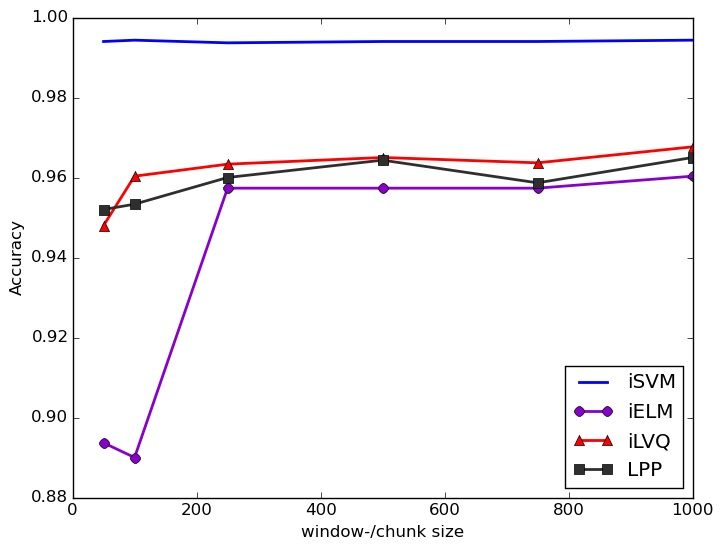
\includegraphics[width=0.47\textwidth]{Images/borderOriginal_random_None_testAccuraciesChunkSizes.jpg}
        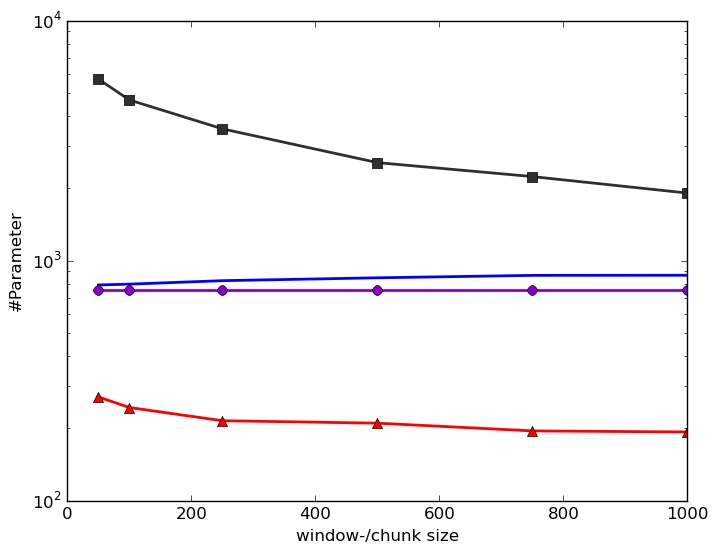
\includegraphics[width=0.47\textwidth]{Images/borderOriginal_random_None_complexityNumParamMetricChunkSizes.jpg}
        \caption{Influence of the window-/chunk size on the accuracy (left) and model complexity (right) for dataset \textit{Border}.}.
        \label{fig:chunkSize}
\end{figure}
Usually the algorithms do benefit from an increased window-/chunk size. For instance, a larger window enables the ILVQ to find better positions for new prototypes and the ISVM to miss less support vectors. 
Simultaneously, the model complexity of ILVQ is reduced since the insertion rate is coupled with the training-error. 
In case of LPP, however, larger chunks reduce the number of base classifiers but at the same time each of them is trained on more training data, requiring a balancing of these criteria.

\subsection{Restriction of the overall classifier complexity}\label{modelComplexity}
Methods as SGD, NB and IELM are on-line algorithms since they are constant in their complexity. ILVQ and LPP can be easily restricted to a certain limit 
by strategies such as removing the ''worst`` prototype/classifier \cite{grbovic2009learning}, \cite{elwell2009incremental}. In case of the ISVM, however, it is less trivial. Even though methods as \cite{Downs:2002:ESS:944790.944814} do reduce the number of support vectors, 
there is to the best of our knowledge no practical method to bound them strictly. This applies to a lesser degree also for the ORF. It learns by growing its trees continuously. Therefore, a depth reduction or pruning mechanism would be necessarily at some point.\\

%The ISVM stores next to the support vectors their $\alpha$ values as well as the intercept resulting in a complexity of $C_{ISVM}=prototypes*(dim+1)+1$. ILVQ stores the prototypes, their labels
%and possibly the metric of the input space $C_{ILVQ}=prototypes*(dim+1)+dim^2$. IELM has the complexity of $C_{IELM}=dim*hneurons+hneurons*classes$
\iffalse
\begin{table}
\centering
\def\arraystretch{0.7}
\footnotesize
\begin{tabular}{c|c<{\hspace{-8pt}}c<{\hspace{-8pt}}c<{\hspace{-8pt}}c<{\hspace{-8pt}}c<{\hspace{-8pt}}c<{\hspace{-8pt}}c<{\hspace{-8pt}}}
& ISVM & ORF & ILVQ & IELM &LPP & GNB & SGD\\\hline
\rule{0pt}{10pt}
\multirow{2}{*}{Border} &265.3   & 1.5k  & 63.0   & 150.0  & 764.7  & -  & \textbf{-} \\
                        &797.0   & 3.7k  & 193.0  & 750.0  & 1.9k   & 12 & \textbf{9} \\


\multirow{2}{*}{Overlap} &3.4k    & 915.3 & 77.0   & 150.0  & 779.3  & -  & \textbf{-} \\
                         &10.0k   & 2.3k  & 235.0  & 900.0  & 1.9k & 16 & \textbf{12} \\

\multirow{2}{*}{Outdoor} &1.8k    & 3.5k  & 463.7   & 200.0  & 2.5k  & -    & \textbf{-} \\
                         &40.0k   & 8.8k  & 10.6k  & 12.2k   & 6.2k  & 1.7k & \textbf{880} \\

\multirow{2}{*}{COIL}    &2.6k   & 24.2k & 796.7   & 300.0  & 3.7k  & -  & \textbf{-} \\
                         &58.1k  & 60.6k & 18.0k   & 36.3k  & 9.2k  & 4.2k & \textbf{2.2k} \\


\multirow{2}{*}{USPS}    &2.8k   & 13.3k & 60.3   & 400.0   & 3.8k  & -     &  \textbf{-} \\
                         &709.8k & 33.3k & 15.1k  & 106.4k  & 9.6k  & 5.1k  &  \textbf{2.6k} \\

\multirow{2}{*}{Letter}  &7.7k   & 67.4k  & 888.3  & 200.0  & 20.4k & -   & \textbf{-} \\
                         &131.1k & 168.5k & 15.4k  & 8.4k  & 51.0k  & 832 & \textbf{442} \\

\multirow{2}{*}{MNist}   &3.2k   & 916  & 71.0   & 150.0  & 770  & -  & \textbf{-} \\
                         &9.7k   & 2.3k & 219.0  & 900.0  & 1.9k & 16 & \textbf{12} \\

\multirow{2}{*}{Gisette} &1.4k   & 1.9k & 52.7   & 500.0   &  \textbf{1.0k}  & -     & - \\
                         &7.0M   & 4.7k & 263.3k & 2.5M    &  \textbf{2.5k}  & 20.0k & 5.0k \\
                        
\multirow{2}{*}{DNA}     &1.3k   & 1.8k   & 3.0   & 300.0  & 657  & -    & \textbf{-} \\
                         &236.6k & 4.5k   & 32.9k & 54.9k  & 1.6k & 1.0k & \textbf{543.0} \\

\multirow{2}{*}{Isolet} &4.6k & 12.4k & 34.7    & 100.0 &  \textbf{4.8k}  & -     & - \\
                        &2.8M & 31.0k & 21.4k   & 64.3k &  \textbf{12.1k} & 32.0k & 16.1k\\\hline
Avg. & 90 \\
Avg. rank \\
\end{tabular}
\caption{Complexities after training with the best chunk-size. The top row of describes the complexity in model specific terms (instances or nodes). Below is the complexity given
in the amount of parameters.}% We neglected the standard deviations since the complexity was stable ($\sigma<1\%$) for all methods. 

\label{tab:complexities}
\end{table}
\fi


\section{Conclusion}
We analyzed the most common algorithms of incremental learning on diverse, stationary datasets. Regarding the results, the ISVM delivers usually the highest accuracy at the expense of the most complex model. 
Its training time is tolerable for tasks consisting of up to 10000 samples. The ORF performs slightly worse but has a very fast training- and
run-time. However, its model as well as those of the ISVM grows linearly with the number of samples and cannot be limited in a straightforward way. Therefore, both algorithms are not suited for learning in endless streams in contrast
to all remaining methods, having either a constant or easily boundable complexity. The ILVQ offers an accurate and sparse alternative to the ISVM. LPP is quite flexible since the base classifier can be arbitrary selected, however,
it may struggle by its limited knowledge integration across chunks. Tree based models are especially suitable for high dimensional data because of their compressed representation as well as their sub-linear run-time, which does not depend on the number of dimensions.
The linear model of SGD is also a good choice for large-scale learning in high dimensional spaces.


% ****************************************************************************
% BIBLIOGRAPHY AREA
% ****************************************************************************

\begin{footnotesize}

\renewcommand{\baselinestretch}{0.6}\footnotesize
\setlength{\bibsep}{0pt}

% IF YOU USE BIBTEX,
% - DELETE THE TEXT BETWEEN THE TWO ABOVE DASHED LINES
% - UNCOMMENT THE NEXT TWO LINES AND REPLACE 'Name_Of_Your_BibFile'

\bibliographystyle{unsrt}
\bibliography{esannV2}

\end{footnotesize}

% ****************************************************************************
% END OF BIBLIOGRAPHY AREA
% ****************************************************************************

\end{document}
